\documentclass[parskip=full]{scrartcl}
\usepackage[utf8]{inputenc} % use utf8 file encoding for TeX sources
\usepackage[T1]{fontenc}    % avoid garbled Unicode text in pdf
\usepackage[english]{babel}  % english hyphenation, quotes, etc
\usepackage{hyperref}       % detailed hyperlink/pdf configuration
\hypersetup{                % ‘texdoc hyperref‘ for options
pdftitle={HePICS: Heterogeneous Platform for Image Classification System},%
bookmarks=true,%
}
\usepackage{graphicx}       % provides commands for including figures
\usepackage{csquotes}       % provides \enquote{} macro for "quotes"
\usepackage{enumitem}


\title{HePICS: Heterogeneous Platform for Image Classification System}

\begin{document}

\maketitle
\thispagestyle{empty}
\pagebreak





\tableofcontents
\pagebreak





\section {Introduction}

This project consists in building an image classification system, which takes images as input and gives a prediction -in percentages- of what would be on these given images. For instance, the system may receive an image of a human face as input, after treating the data, the output is then represented in a small list of objects that may be on the picture, ordered by their probability percentages. In this case, the system should display a list, whose first element "human face" is, next to the probability which the system calculated for this result.

The motivation behind this project is artificial neural networks. These are computing systems which were inspired by the biological neural network of an animal. Such systems gain knowledge in executing tasks -in our case image recognition- through a certain training. For an image recognition neural network to correctly perform its task, it is required to analyze examples of images that have been manually labeled. Other uses where artificial neural networks are deployed are predictions, function approximations, or real life patterns recognition...

Nowadays, machine learning is gaining in importance as the goal of including machines in various activities -industries, services, economy- in order to reach high levels of efficiency is in need of artificial intelligence. Indeed, under the applications of artificial neural networks, we can mention autonomous driving, natural language processing, gesture recognition, and of course, face recognition, which is the main application of this project.

It must not be forgotten to mention as well, that there exists different neural networks models, such as Back-Propagation, Boltzmann Machines and Deep Neural Networks, with which we will deal in this project. In particular, we will deal with "AlexNet", which is a convolutional neural network consisting of 8 layers, 5 of which are convolutional while the others are fully-connected layers.

On one hand, deploying deep neural networks not only means unlocking a massive parallelism potential for our system, but it also means that unsupervised learning is most definitely possible. On the other, we are in need of a huge data set for this unsupervised training. It is important to mention as well, that deep neural networks require intense computations, which manifests itself in high power consumption and learning and classification time.

For the sake of decreasing the number of disadvantages of deep neural networks, the decision of using heterogeneous platforms such as CPUs, GPUs and FPGAs was made. These will provide the system with a good performance for a wide range of computations, as well as a decent usage of pipelines and parallelism, and of course, all with low power consumption.

To take a taste at the fascinating world of machine learning and artificial neural networks, we invite you to try out our image recognition system, and maybe even have a little fun with it.

\pagebreak





\section{Target specifications}

\subsection{Must-requirements}

\begin{itemize}
	\item The system must be able to classify images.
	\item The system must allow the selection of one or more input images.
	\item The system must show the result of the treatment.
	\item The system must employ artificial neural networks.
	\item The system must deploy the AlexNet deep neural network.
	\item The system must know at least one set of weights.
	\item The system must be able to execute intense calculations through heterogeneous platforms (CPU, GPU, FPGA, ASIC).
	\item The system must support an FPGA through OpenCL.
	\item The system must hide the OpenCL details behind an abstraction layer.
	\item The system must offer three performance profiles : 
	\begin{itemize}
		\item High Performance
		\item Low Power
		\item Energy Efficency
	\end{itemize}
	\item The system must allow the control and the execution of commands through a GUI interface.
	\item The system must be able to run the GUI on an Ubuntu system.
	\item The system must exhibit a classification interface.
	\item The system must be able to measure its performance.
	\item The system must be able to measure its power consumption.
	\item The system communicate with another system. It looks into a file to search for an image treatment request, and send back the results via Ethernet connection.
	\item The system be able to run in batch processing mode.
	\item The system must include the aggregate feature. This feature fuses the results of different treatments of the same object in order to reach more precision.
	\item The system must offer the possibility of entering up to 5 images in the aggregate feature.
\end{itemize}

\subsection{Can-Requirements}

\begin{itemize}
	\item The system can offer the possibility of entering more than 5 images in the aggregate feature.
	\item The system can deploy a GPU.
	\item The system can deploy a DSP.
	\item The system can deploy an ASIC (Movidius Stick).
	\item The system can deploy the GoogleNet neural network next to AlexNet. 
	\item The system can allow the training of neural networks.
	\item The system can display the topology of the neural network.
	\item The system can write the results into a file in order to use it for another program.
	\item The system can carry out transfer learning of the already implemented neural network.
	\item The system can beautify the output result.
	\item The system can generate weight files.
	\item The system can load different weight files.
	\item The system can pause, resume or cancel the classification process.
\end{itemize}

\subsection{Criteria of demarcation}

\begin{itemize}
	\item The system cannot be a real-time application.
	\item The system cannot run on mobile-plattforms.
\end{itemize}

\pagebreak






\section{Product Use}

\subsection{Field of application}
 
This program is designed for image classification. The user or system can use this program to recognize pre-specified or learned objects. Because the system runs on heterogeneous platforms, the user is allowed to switch between various operation modes depending on power or performance preferences.

Victims of strokes or memory problems have a hard time recognizing even the most simple objects we deal with everyday. Building on this system, it would be possible to help these people to rebuild their memories or label the objects presented on the images. It can also help the visually disabled have a better idea about their environment through processing images they choose.
Another application of this system is the optimization of the traffic lights through equipping them with a functionality that would set the traffic free for other sides, if the current side is empty.

We can think about a use in the tourism field as well, as tourists may want to have a better idea about buildings or statues of the city they are visiting, which they can do through our system.

\subsection{Target Group}

\begin{itemize}
	\item people with impaired vision
	\item tourists
	\item developers of other systems
	\item users who need to classify images
	\item systems which process images or solve problem in computer vision
\end{itemize}

\pagebreak



\subsection{Operation Condition}

The following conditions must be met:

\begin{itemize}
	\item Hardware and software as follows must be available: 
	\begin{itemize}
		\item Host PC with Ubuntu 16.04
		\item FPGA
	\end{itemize}
	\item System and possible user-system must be installed.
	\item Images must be accessible to file system.
	\item Host PC must be powered.
	\item FPGA must be powered.
	\item Images must be JPG.
	\item FPGA have to be connected to Host PC.
	\item There must be enough storage for the program.
	\item There must be enough storage to store results. 
\end{itemize}

\pagebreak





\section{Product Environment}

\subsection{Software}

\begin{itemize}
	\item Ubuntu 16.04 - operating system of Host PC
	\item QT - to create classic and embedded GUI
	\item OpenCL - framework for writing programs that execute across heterogeneous platforms
\end{itemize}

\subsection{Hardware}

\begin{itemize}
	\item Desktop PC
	\item DE1SoC (SOC that includes FPGA)
\end{itemize}
 
\pagebreak





\section{Product Functions} \label {pfunc}

\subsection{Basic Functions} \label {bfunc}

\begin{itemize}
	\item[/F010/] Show welcome window.
	\item[/F020/] Show main window. 
	\item[/F030/] Choose input image(s).
	\item[/F040/] Remove single image from the selection.
	\item[/F050/] Show thumbnail of the selected image.
	\item[/F060/] Reset the selection of the images.
	\item[/F065/] Choose platform:
	\begin{itemize}
		\item CPU
		\item FPGA
		\item GPU
		\item ASIC
	\end{itemize}
	\item[/F070/] Choose operation mode: 
	\begin{itemize}
		\item High Performance
		\item Low Power Consumption
		\item High Energy Efficiency
	\end{itemize}
	\item[/F080/] Change the operation mode before starting processing.
	\item[/F090/] Block parts of GUI.
	\item[/F100/] Start processing.
	\item[/F110/] Pause processing.
	\item[/F120/] Resume processing.
	\item[/F130/] Cancel processing.
	\item[/F140/] Switch between start button and cancel button.
	\item[/F150/] Switch between pause button and resume button.
	\item[/F160/] Run calculation through FPGA.
	\item[/F170/] Aggregate results of multiple images.
	\item[/F180/] Show output results (names and percentages of top 4).
	\item[/F190/] Terminate program.
	\item[/F200/] Start a new classification.
	\item[/F210/] Poll the request file from another system.
	\item[/F220/] Send back the results via Ethernet.

\end{itemize}

\subsection{Optional Functions} \label {ofunc}

\begin{itemize}
	\item[/F230/] Run calculation through GPU.
	\item[/F240/] Run calculation through ASIC.
	\item[/F250/] Choose the neural network topology.
	\item[/F260/] Show the neural network topology.
	\item[/F270/] Deploy training of an arbitrary neural network.
	\item[/F280/] Transfer learning of the already implemented neural network.
	\item[/F290/] Show a progress bar while classifying.
	\item[/F300/] Show output results in clear form (with a histogram).
	\item[/F310/] Write output results into a new file.
\end{itemize}

\pagebreak





\section{Product-Data}

\subsection{System-Data}

\begin{itemize}
	\item[/D10/] Classification results with percentage bars.
	\item[/D20/] The nodes' weight files.
	\item[/D30/] The neural network's topology.
\end{itemize}

\subsection{User-Data}

\begin{itemize}
	\item[/D40/] The input images are saved.
	\item[/D50/] The results are saved.
\end{itemize}

\pagebreak





\section{System Model}

Programming with less complexity makes delightful code that is less buggy and easier to maintain because it is reusable without modification. In order to achieve this goal we use in this context the MVC architecture which consists of three parts: Model, View and Controller.

\begin{center}
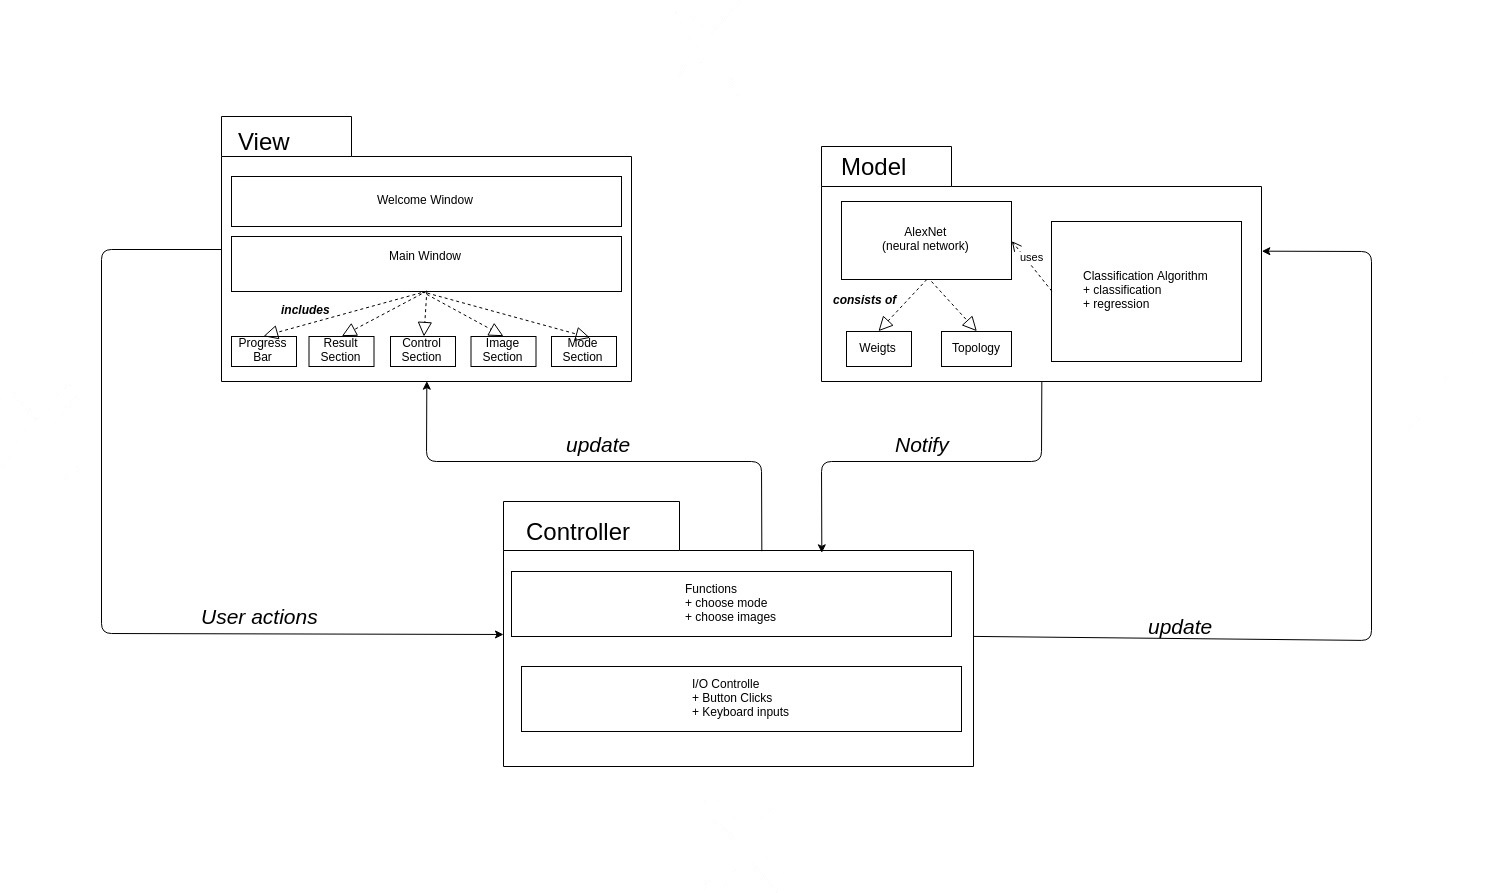
\includegraphics[width=1.0\textwidth]{images/MVC.png}
\end{center}

\subsection{Model}

The model represents the domain. The model does not depend on the controller or the view. It contains the pretrained neural network model AlexNet as well as the classification algorithm to be used on images.The neural network itself is composed of a set of weights and topology. The topology sepecifies how the layers interact with each other. On the other hand the weights define when the neurons are activated. The layers are invoked by the scheduler which is responsible for resolving dependencies between them.

\pagebreak



\subsection{View}

The view displays the model data. The model data is in this case the input images,  the output results and the chosen operation mode as well as the current state of the process (e.g. in pause, running, waiting for input). Besides it sends user actions (e.g. button clicks, inputs) to the controller. It represents the graphical user interface which allows the user to interact with the system (See Graphical User Interface)

\subsection{Controller}

The controller interprets user actions such as button clicks. It depends on the view and the model and controls the interactions between them.

\pagebreak





\subsection{Use Cases}


\subsubsection {Use Case: Select single image}

\begin{enumerate}
	\item Preface
	\begin{itemize} [nosep]
		\item[] Primary Actor: User
	\end{itemize}
	\item Stakeholders and Interest
	\begin{itemize} [nosep]
		\item[] User : wants the classification of an image through selecting one single image as an input, and needs the result showed in a clear form, without any errors.
	\end{itemize}
	\item Preconditions
	\begin{itemize} [nosep]
		\item[] The system is started, the welcome screen is showed, the main window loads correctly.
	\end{itemize}
	\item Post conditions
	\begin{itemize} [nosep]
		\item[] The input image is correctly selected. The thumbnail of the image is showed on the screen with the possibility of removing it. The start button is active and the classification can be started.
	\end{itemize}
	\item Main Success Scenario
	\begin{itemize} [nosep]
		\item[1.] User starts the program.
		\item[2.] Welcome screen is displayed.
		\item[3.] User clicks on the "start" button.
		\item[4.] Main window is displayed.
		\item[5.] User clicks on a "add image..." button.
		\item[6.] User selects an image.
		\item[7.] System loads image file.
		\item[8.] Selected image's thumbnail is displayed and start button is activated.
	\end{itemize}
	\item Extensions
	\begin{itemize} [nosep]
		\item[*a.] At any time, system fails :
		\begin{itemize} [nosep]
			\item[1.] System signals error to the user, records the error and enters a clean state.
			\item[2.] System reloads the main window. 6a. Invalid input image
			\item[3.] System signals the invalid input and rejects it
			\item[4.] User selects a new input image, or cancels the selection.
		\end{itemize}
	\end{itemize}
\end{enumerate}

\pagebreak



\subsubsection {Use Case: Select multiple images}

\begin{enumerate}
	\item Preface
	\begin{itemize} [nosep]
		\item[] Primary Actor: User
	\end{itemize}
	\item Stakeholders and Interest
	\begin{itemize} [nosep]
		\item[] User: Wants to classify objects more accurately by providing multiple images.showed in a clear form, without any errors.
	\end{itemize}
	\item Preconditions
	\begin{itemize} [nosep]
		\item[] Image classification system is running. The user prepared multiple images of the same object he wants to classify.
	\end{itemize}
	\item Post conditions
	\begin{itemize} [nosep]
		\item[] Images are accessible to the system.
	\end{itemize}
	\item Main Success Scenario
	\begin{itemize} [nosep]
		\item[1.] User starts the program.
		\item[2.] Welcome screen is displayed.
		\item[3.] User clicks on the "start" button.
		\item[4.] Main window is displayed.
		\item[5.] User clicks on a "add image..." button.
		\item[6.] User selects an image.
		\item[7.] Selected image's thumbnail is displayed and start button is activated.
		\item[8.] User repeats step 5-6.
	\end{itemize}
	\item Extensions
	\begin{itemize} [nosep]
		\item[*a] The selection is reset.
			\begin{itemize} [nosep]
				\item[1.] The system initializes the selection state.
			\end{itemize}
		\item[6a.] The extension name of file isn't supported.:
		\begin{itemize} [nosep]
			\item[1.] System signals error and displays it on the screen.
		\end{itemize}
		\item[7a] One of the images is removed.
		\begin{itemize} [nosep]
			\item[1.] System signals error to the user, records the error and enters a clean state.
		\end{itemize}		
	\end{itemize}
\end{enumerate}

\pagebreak


\subsubsection {Use Case: Send input image} \label {uc:sip}

\begin{enumerate}
	\item Preface
	\begin{itemize} [nosep]
		\item[] Primary Actor: External system
	\end{itemize}
	\item Stakeholders and Interest
	\begin{itemize} [nosep]
		\item[] External systems human user: Wants external system to provide its service fast, accurate and energy efficient.
	\end{itemize}
	\item Preconditions
	\begin{itemize} [nosep]
		\item[] External system and image classification system are running.
		\item[] The external system must be connected to the image classification system.
		\item[] The external system must be able to write the request file.
	\end{itemize}
	\item Post conditions
	\begin{itemize} [nosep]
		\item[] The image classification system has access to the images to be classified.
	\end{itemize}
	\item Main Success Scenario
	\begin{itemize} [nosep]
		\item[1.] User runs external system.
		\item[2.] External system sends image file to filesystem of image classification system.
		\item[3.] External system repeats 2 until done.
	\end{itemize}
	\item Extensions
	\begin{itemize} [nosep]
		\item[*a.] At any time, image classification system is shut down:
		\begin{itemize} [nosep]
			\item[1.] A shut down signal is sent.
		\end{itemize}
	\end{itemize}
\end{enumerate}

\pagebreak



\subsubsection {Use Case: Give classification request}

\begin{enumerate}
	\item Preface
	\begin{itemize} [nosep]
		\item[] Primary Actor: External system
	\end{itemize}
	\item Stakeholders and Interest
	\begin{itemize} [nosep]
		\item[] External systems human user: Wants external system to provide its service fast, accurate and energy efficient.
	\end{itemize}
	\item Preconditions
	\begin{itemize} [nosep]
		\item[] Input images were sent as described in use case \ref {uc:sip} and are accessible.
	\end{itemize}
	\item Post conditions
	\begin{itemize} [nosep]
		\item[] The request was accepted.
	\end{itemize}
	\item Main Success Scenario
	\begin{itemize} [nosep]
		\item[1.] Input images were sent.
		\item[2.] External system writes command to request file.
		\item[3.] Image classification system reads request file.
		\item[4.] Image classification system accepts the request.
	\end{itemize}
	\item Extensions
	\begin{itemize} [nosep]
		\item[*a.] At any time, image classification system is shut down:
		\begin{itemize} [nosep]
			\item[1.] A shut down signal is sent.
		\end{itemize}
		\item[3a.] The request is invalid:
		\begin{itemize} [nosep]
			\item[1.] An error signal is sent.
		\end{itemize}
	\end{itemize}
\end{enumerate}

\pagebreak

\subsubsection {Use Case: Select operation mode}

\begin{enumerate}
	\item Preface
	\begin{itemize} [nosep]
		\item[] Primary Actor: User
	\end{itemize}
	\item Stakeholders and Interest
	\begin{itemize} [nosep]
		\item[] User: Wants fast and accurate selection of the operation mode. Wants fast update of the mode when changing selection.
	\end{itemize}
	\item Preconditions
	\begin{itemize} [nosep]
		\item[] The Classification system is started.
		\item[] Main window is displayed
	\end{itemize}
	\item Post conditions
	\begin{itemize} [nosep]
		\item[] The system is aware of the chosen mode.
	\end{itemize}
	\item Main Success Scenario
	\begin{itemize} [nosep]
		\item[1.] User starts the application.
		\item[2.] Welcome window is displayed.
		\item[3.] User clicks on start.
		\item[4.] Main window is displayed.
		\item[5.] User selects operation mode by selecting it in the dropdown menu.
	\end{itemize}
	\item Extensions
	\begin{itemize} [nosep]
		\item[*a.] At any time, image classification system is shut down:
		\begin{itemize} [nosep]
			\item[1.] User chooses the operation mode again.
			\item[2.] User selects images again.
			\item[3.] User restarts the process.
		\end{itemize}
		\item[5a.] User cannot switch to another operation mode
		\begin{itemize} [nosep]
			\item[1.] System restarts.
		\end{itemize}
	\end{itemize}
\end{enumerate}

\pagebreak



\subsubsection {Use Case: Classify Image}

\begin{enumerate}
	\item Preface
	\begin{itemize} [nosep]
		\item[] Primary Actor: User, External system
	\end{itemize}
	\item Stakeholders and Interest
	\begin{itemize} [nosep]
		\item[] User: Wants images to be classified accurately and fast.
		\item[] External System: Wants images to be classified accurately
	\end{itemize}
	\item Preconditions
	\begin{itemize} [nosep]
		\item[] Input images were sent by the external system or the user loaded the images.
		\item[] The operation mode was selected.
		\item[] The weight file to be used is already available to the system.
	\end{itemize}
	\item Post conditions
	\begin{itemize} [nosep]
		\item[] The classification process is successfully terminated.
	\end{itemize}
	\item Main Success Scenario
	\begin{itemize} [nosep]
		\item[1.] Classification process terminates.
		\item[2.] System displays results on the main window.
		\item[3.] System saves results in a file (for external systems).
		\item[4.] System sends the file with results to the external system.
	\end{itemize}

\pagebreak

	\item Extensions
	\begin{itemize} [nosep]
		\item[*a.] Classification process fails to terminate.
		\begin{itemize} [nosep]
			\item[1.] User chooses the operation mode again.
			\item[2.] User selects images again.
			\item[3.] User restarts the process.
		\end{itemize}
		\item[2a.] Program fails to display results.
		\begin{itemize} [nosep]
			\item[1.] User chooses the operation mode again.
			\item[2.] User selects images again.
			\item[3.] User restarts the process.
		\end{itemize}
		\item[4a.] File was not sent due to bad connection.
		\begin{itemize} [nosep]
			\item[1.] Check connection with the external system.
			\item[1.] Reset Connection.
			\item[1.] Send the file again.
		\end{itemize}
		\item[4b.] File was not sent because the file was not saved at all.
		\begin{itemize} [nosep]
			\item[1.] Restart process again.
		\end{itemize}
	\end{itemize}
\end{enumerate}

\pagebreak

\subsubsection {Use Case: Get Results}

\begin{enumerate}
	\item Preface
	\begin{itemize} [nosep]
		\item[] Primary Actor: External system
	\end{itemize}
	\item Stakeholders and Interest
	\begin{itemize} [nosep]
		\item[] External system : wants the classification of an image through sending one single request, and needs the result in a clear form, without any errors. Receives then the results through Ethernet. 
		\item[] User of the external system : sends a request through the external system and awaits for the correct and clear results of his request.
	\end{itemize}
	\item Preconditions
	\begin{itemize} [nosep]
		\item[] External system gives request through sending an input image.
		\item[] System detects request.
		\item[] System loads the image and starts classifying it.
		\item[] The classification should run smoothly and be finished.
	\end{itemize}
	\item Post conditions
	\begin{itemize} [nosep]
		\item[] The sent input image is correctly classified. 
		\item[] The results are saved into a file. 
		\item[] The file is sent to the external system.
	\end{itemize}
	\item Main Success Scenario
	\begin{itemize} [nosep]
		\item[1.] User sends an input image through the external system.
		\item[2.] Image classification system detects the classification request.
		\item[3.] System loads the input image.
		\item[4.] System starts the classification.
		\item[5.] System shows results.
		\item[6.] System saves results into a file.
		\item[7.] System sends file to the external system.
	\end{itemize}

\pagebreak

	\item Extensions
	\begin{itemize} [nosep]
		\item[*a.] At any time, image classification system is shut down:
		\begin{itemize} [nosep]
			\item[1.] System restarts, signals error to the external system, records the error, and enters a clean state.
			\item[2.] System loads in input image and restarts classification
		\end{itemize}
		\item[2a] Invalid input image :
		\begin{itemize} [nosep]
			\item[1.] System signals the invalid input and rejects it.
		\end{itemize}
		\item[6a] Saving failed : 
		\begin{itemize} [nosep]
			\item[1.] System signals fail.
			\item[1.] System retries saving file.
		\end{itemize}				
	\end{itemize}
	\item Special Requirements
	\begin{itemize} [nosep]
		\item Ethernet connection between the system and the external system to allow file sharing.
		\item System runs per default on high-efficiency mode.
	\end{itemize}
	\item Technology and Data variations
	\begin{itemize} [nosep]
		\item Results are saved into a text file.
	\end{itemize}
	
\end{enumerate}

\pagebreak

\subsubsection {Use Case: View Results }

\begin{enumerate}
	\item Preface
	\begin{itemize} [nosep]
		\item[] Primary Actor: User
	\end{itemize}
	\item Stakeholders and Interest
	\begin{itemize} [nosep]
		\item[] User : wants to get results of the classification.
	\end{itemize}
	\item Preconditions
	\begin{itemize} [nosep]
		\item[] The processing of classification was finished successfully. The system aggregated the results of multiple images.
	\end{itemize}
	\item Post conditions
	\begin{itemize} [nosep]
		\item[] The results are displayed successfully. The new file with results is accessible to the user.
	\end{itemize}
	\item Main Success Scenario
	\begin{itemize} [nosep]
		\item[1.] User selects image(s).
		\item[2.] System starts classification.
		\item[3.] System finishes classification.
		\item[4.] User views results on the main window. 
		\item[5.] User selects image to view specific results. 
	\end{itemize}
	\item Extensions
	\begin{itemize} [nosep]
		\item[*a.] At any time, system fails :
		\begin{itemize} [nosep]
			\item[1.] System signals error to the user, records the error and enters a clean state.
			\item[2.] System reloads the main window.
		\end{itemize}
		\item[4a] The user wants a new file containing the results.
		\begin{itemize} [nosep]
			\item[1.] System saves results into a file.
		\end{itemize}
	\end{itemize}
\end{enumerate}

\pagebreak



\subsubsection {Use Case: Aggregate results }

\begin{enumerate}
	\item Preface
	\begin{itemize} [nosep]
		\item[] Primary Actor: User
	\end{itemize}
	\item Stakeholders and Interest
	\begin{itemize} [nosep]
		\item[] User: wants the result of the classification of multiple images he selects. This result is an aggregation of the results of each image.
	\end{itemize}
	\item Preconditions
	\begin{itemize} [nosep]
		\item[] The selection of up to 5 images runs correctly. The classification of each image is correctly executed.
	\end{itemize}
	\item Post conditions
	\begin{itemize} [nosep]
		\item[] The results of each image are aggregated creating a new result. This new result is displayed on the main window.
	\end{itemize}
	\item Main Success Scenario
	\begin{itemize} [nosep]
		\item[1.] User starts program.
		\item[2.] User adds one image.
		\item[3.] User adds more images.
		\item[4.] System starts the classification.
		\item[5.] System finishes the classification.
		\item[6.] System starts the aggregation.
		\item[7.] System shows the aggregation results.
	\end{itemize}
	\item Extensions
	\begin{itemize} [nosep]
		\item[*a.] At any time, system fails :
		\begin{itemize} [nosep]
			\item[1.] System signals error to the user, restarts, records the error, and enters a clean state.
			\item[2.] System loads in input images and restarts classification.
		\end{itemize}
		\item[2-3a] Invalid input image :
		\begin{itemize} [nosep]
			\item System signals the invalid input and rejects it.
		\end{itemize}
	\end{itemize}
\end{enumerate}



\subsection {Use Case Diagrams}

The section contains the use case diagrams. They show how the use cases are related to each other.

\subsubsection {Simple Usage}

The diagram shows a simple classification of a single image. 

\begin{center}
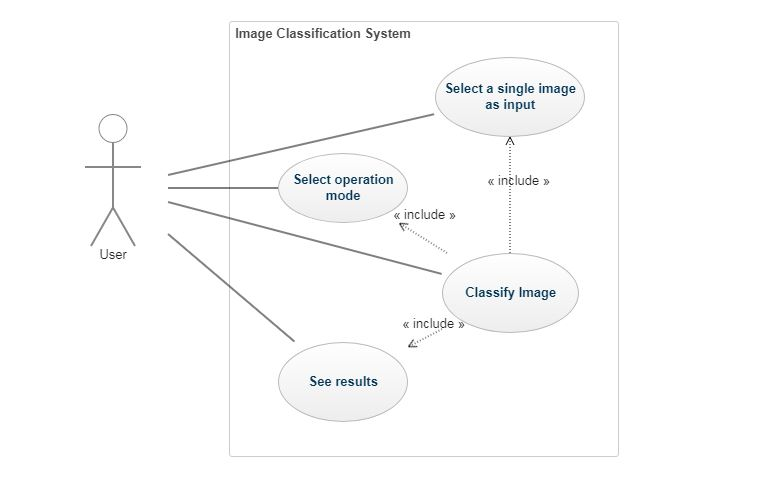
\includegraphics[width=1.0\textwidth]{UseCases/NormalUsageUCD.JPG}
\end{center}

\pagebreak



\subsubsection {Aggregated Results Usage}

The diagram shows a classification that aggregates the results of multiple images. 

\begin{center}
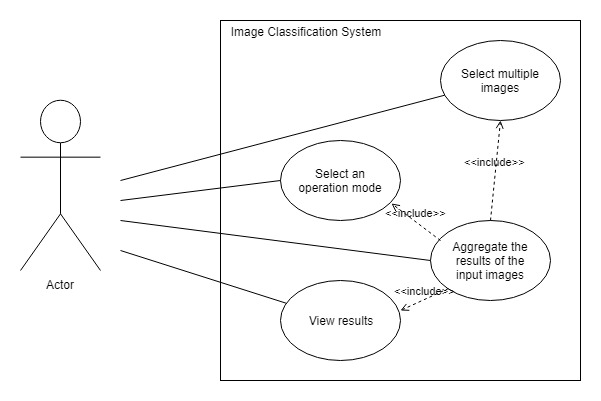
\includegraphics[width=0.8\textwidth]{UseCases/AggregateUCD.jpg}
\end{center}

\pagebreak



\subsubsection {Usage by an External System}

The diagram shows how an external system runs a classification. 

\begin{center}
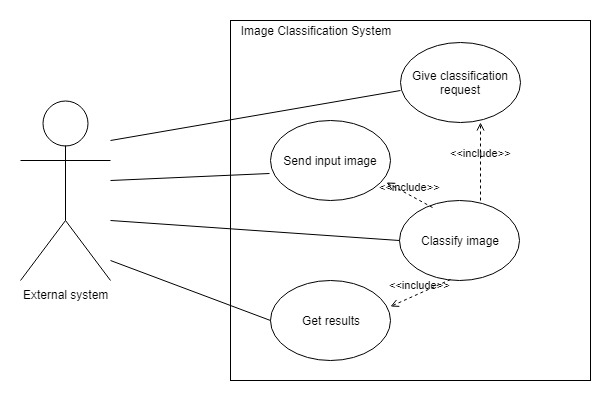
\includegraphics[width=0.8\textwidth]{UseCases/ExtenalSystemUCD.jpg}
\end{center}

\pagebreak





\section{Product Performance}

\begin{itemize}
	\item[/P010/] The user clicks on a start button in order to start the program.
	\item[/P020/] The user chooses the operation mode with two clicks.
	\item[/P030/] The user switches between operation modes in two clicks.
	\item[/P040/] The user uploads an image in a maximum of three clicks.
	\item[/P050/] The user removes an image in three clicks.
	\item[/P060/] The user resets the selection in one button.
	\item[/P070/] The system shows a progress bar while classifying.
	\item[/P080/] The user pauses the process in one click.
	\item[/P090/] The user resumes the process in one click.
	\item[/P100/] The user cancels the process in a maximum of three buttons.
	\item[/P110/] The user exits the program in a maximum of three buttons.
	\item[/P120/] The user starts a new classification in a maximum of three buttons.
	\item[/P130/] Low Power Consumption Mode should consume the least amount of power.
	\item[/P140/] High Performance Mode should execute the fastest.
	\item[/P150/] High Energy Efficiency Mode is the most power consumption and time efficient of the three modes.
\end{itemize}

\pagebreak





\section {Graphical User Interface}

The GUI, which represents the front-end, is the communication channel between the user and the back-end (the internal system). It will guide users through the variety of operations which can be performed by the System.

\subsection {Welcome-Window}

After the program starts, a welcome window with information on the Software will be displayed. This information consists of a short description of the  system and the current version of the software.

\begin{center}
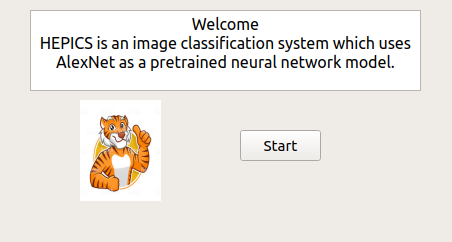
\includegraphics[width=1.0\textwidth]{images/WelcomeWindow.png}
\end{center}

\pagebreak



\subsection {Main-Window}

After clicking on Start-button in the welcome window, another window will pop up. It is called main window. The main window contains multiple sections.

\begin{center}
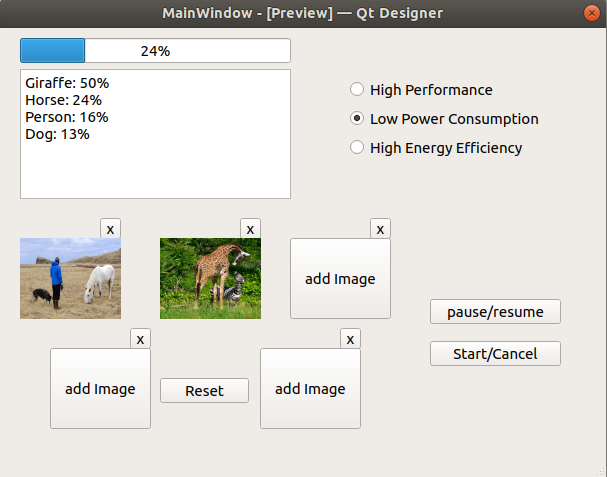
\includegraphics[width=1.0\textwidth]{images/MainWindow.png}
\end{center}

\pagebreak



\subsubsection {Choose-Operation-Section}

 The user has to choose a running mode:

\begin{enumerate}
	\item High Performance
	\item Low Power Consumption
	\item High Energy Efficiency
\end{enumerate}

\begin{center}
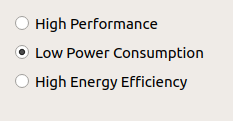
\includegraphics[width=0.5\textwidth]{images/ChooseOperationMode.png}
\end{center}

\subsubsection {Result-Section}

The result section contains results of aggregation. The results are represented in form of text. The results are the probabilities of the top detected objects in percentages.

\begin{center}
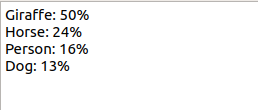
\includegraphics[width=0.5\textwidth]{images/ResultSection.png}
\end{center}

\subsubsection {Progress-Bar}

The progress bar shows the state of the current running process.

\begin{center}

\includegraphics[width=0.5\textwidth]{images/ProgressBar.png}
\end{center}

\pagebreak



\subsubsection {Image-Section}

The image section consists of multiple buttons which can be used to add images. Thumbnails are generated afterwards and will be displayed on the buttons. An image can be removed through clicking on the remove-button. All images can also be removed at once if the user clicks on the reset-button.

\begin{center}
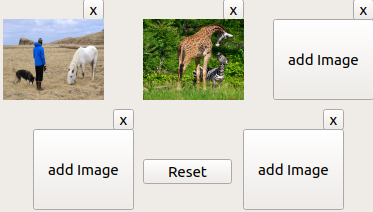
\includegraphics[width=0.9\textwidth]{images/ImageSection.png}
\end{center}

\subsubsection {Control-Section}

By using the control section the user is able to start and cancel the process. Once the classification starts, the start button becomes a cancel button. While running the user can pause the classification by clicking on the pause button. In this case the pause button becomes a resume button.

\begin{center}
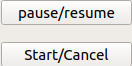
\includegraphics[width=0.3\textwidth]{images/ControlSection.png}
\end{center}

\pagebreak





\section {Test Cases}

All functions are tested by the following test cases. The basic tests test the basic functions. The extended tests test the optional functions. The actions described here are atomic from a users point of view.

\subsection {Basic tests}

\begin{itemize}
	\item[/T010/] Start application. (/F010/, /F090/, \ref{bfunc})
	\item[/T020/] Press start on welcome screen. (/F020/, \ref{bfunc})
	\item[/T030/] Start file open dialog for image. (/F030/, \ref{bfunc})
	\item[/T040/] Choose image file. (/F030/, /F050/, \ref{bfunc})
	\item[/T050/] Choose a file, whose format is not supported. (/F030/, \ref{bfunc})
	\item[/T060/] Choose multiple input image files. (/F030/, \ref{bfunc})
	\item[/T070/] Abort image file selection. (/F030/, \ref{bfunc})
	\item[/T080/] Remove a selected image. (/F040/, \ref{bfunc})
	\item[/T090/] Reset the selection of images. (/F060/, \ref{bfunc})
	\item[/T100/] Choose operation mode high performance. (/F070/, /F080/, \ref{bfunc})
	\item[/T110/] Choose operation mode low power consumption. (/F070/, /F080/, \ref{bfunc})
	\item[/T120/] Choose operation mode high energy efficiency. (/F070/, /F080/, \ref{bfunc})
	\item[/T130/] Start processing. (/F100/, /F090/, /F140/, /F160/, \ref{bfunc})
	\item[/T140/] Pause processing. (/F110/, /F150/, \ref{bfunc})
	\item[/T150/] Resume processing. (/F120/, /F150/, \ref{bfunc})
	\item[/T160/] Cancel processing. (/F130/, /F140/, \ref{bfunc})
	\item[/T170/] Finish processing. (/F090/, /F140/, /F170/, /F180/, \ref{bfunc})
	\item[/T180/] Close program. (/F190/, \ref{bfunc})
	\item[/T190/] Start new classification. (/F200/, \ref{bfunc})
	\item[/T200/] Receive a classification request in the request file. (/F210/, /F220/, \ref{bfunc})
\end{itemize}

\pagebreak



\subsection {Extended tests}

\begin{itemize}
	\item[/T210/] Start processing. (/F230/, /F240/, /F290/, \ref{ofunc})
	\item[/T220/] Finish processing. (/F300/, /F310/, \ref{ofunc})
	\item[/T230/] Start file open dialog for topology. (/F250/, \ref{ofunc})
	\item[/T240/] Choose topology. (/F250/, \ref{ofunc})
	\item[/T250/] When choosing a topology choose a non topology file. (/F250/, \ref{ofunc})
	\item[/T260/] Press show topology button. (/F260/, \ref{ofunc})
	\item[/T270/] Start file open dialog for weights. (/F270/, \ref{ofunc})
	\item[/T280/] Choose weights. (/F270/, \ref{ofunc})
	\item[/T290/] When choosing weights choose a non weights file. (/F270/, \ref{ofunc})
	\item[/T300/] Choose weights for another topology (/F270/, \ref{ofunc})
	\item[/T310/] Choose AlexNet (/F270/, \ref{ofunc})
	\item[/T320/] Choose GoogleNet (/F270/, \ref{ofunc})
	\item[/T330/] Run transfer learning (/F280/, \ref{ofunc})
\end{itemize}

\pagebreak





\section{Test Scenarios}

The test scenarios consist of the test cases listed above.

\subsection {Scenario: Select multiple images}

\begin{enumerate}
	\item /T010/ Start application. 
	\item /T020/ Press start on welcome screen.
	\item /T030/ Start file open dialog for image.
	\item /T040/ Choose image file.
	\item /T050/ Choose a file, whose format is not supported.
	\item /T040/ Choose image file.
	\item /T080/ Remove a selected image.
	\item /T090/ Reset the selection of images. 
	\item /T060/ Choose multiple input image files.
	\item /T100/ Choose operation mode high performance.
	\item /T130/ Start processing.
	\item /T170/ Finish processing.
	\item /T180/ Close program.
\end{enumerate}

\pagebreak



\subsection {Scenario: View Results}

\begin{enumerate}
	\item /T010/ Start application.  
	\item /T020/ Press start on welcome screen.
	\item /T030/ Start file open dialog for image.
	\item /T040/ Choose image file.
	\item /T110/ Choose operation mode low power consumption.
	\item /T130/ Start processing.
	\item /T170/ Finish processing.
	\item /T180/ Close program.
\end{enumerate}

\pagebreak

\subsection {Scenario: Give Classification Results}

\begin{enumerate}
	\item /T010/ Start application. 
	\item /T020/ Press start on welcome screen.
	\item /T200/ Receive a classification request in the request file.
	\item /T120/ Choose operation mode high energy efficiency.
	\item /T130/ Start processing.
	\item /T170/ Finish processing.
	\item /T190/ Start new classification
\end{enumerate}

\subsection {Scenario: Send input image}

\begin{enumerate}
	\item /T010/ Start application. 
	\item /T020/ Press start on welcome screen.
	\item /T200/ Receive a classification request in the request file.
\end{enumerate}

\pagebreak


\subsection {Scenario: Select operation mode}

\begin{enumerate}
	\item /T010/ Start Application.
	\item /T020/ Press Start on Welcome screen.
	\item Choose one of the following
	\begin{enumerate}
		\item /T100/ Choose operation mode high performance.
		\item /T110/ Choose operation mode low power consumption.
		\item /T120/ Choose operation mode high energy efficiency.
	\end{enumerate}
	\item Choose one of the following
	\begin{enumerate}
		\item /T060/ Choose multiple input image files.
		\item /T040/ Choose image file.
	\end{enumerate}
	\item /T130/ Start processing.
\end{enumerate}

\pagebreak



\subsection {Scenario: Classify Image}

\begin{enumerate}
	\item /T010/ Start Application.
	\item /T020/ Press Start on Welcome screen.
	\item Choose one of the following
	\begin{enumerate}
		\item /T100/ Choose operation mode high performance.
		\item /T110/ Choose operation mode low power consumption.
		\item /T120/ Choose operation mode high energy efficiency.
	\end{enumerate}
	\item /T040/ Choose image file.
	\item /T140/ Pause processing.
	\item /T150/ Resume processing.
	\item Choose one of the following
	\begin{enumerate}
		\item /T170/Finish processing.
		\item /T160/ Cancel processing.
	\end{enumerate}
\end{enumerate}

\subsection {Scenario: Give Classification Request}

\begin{enumerate}
	\item /T010/ Start application.  
	\item /T020/ Press start on welcome screen.
	\item /T200/ Receive a classification request in the request file.
\end{enumerate}

\pagebreak



\section{Development Environment}

\subsection {Software}

\begin{itemize}
	\item Operating system
	\begin{itemize}
		\item Ubuntu 16.04
	\end{itemize}
	\item Development tools
	\begin{itemize}
		\item Eclipse
		\item Eclipse CDT
		\item Gcov
		\item Boost
		\item Qt
		\item Qt Designer
		\item Altera SDK for OpenCL
	\end{itemize}
	\item Version-control
	\begin{itemize}
		\item Git
	\end{itemize}
	\item Documentation
	\begin{itemize}
		\item Markdown
		\item Latex
	\end{itemize}
\end{itemize}

\subsection {Hardware}

\begin{itemize}
	\item Desktop PC (x64 based)
	\item DE1SoC (SOC that includes an FPGA)
\end{itemize}

\pagebreak


\section{Glossary}
\begin{itemize}
	\item Neural Network:
	\begin{itemize}
		\item Artificial neural networks (ANN) are computing systems vaguely inspired by the biological neural networks that constitute animal brains. The neural network itself is a framework for many different machine learning algorithms to work together and process complex data inputs.
	\end{itemize}
	
	
	\item AlexNet
	\begin{itemize}
		\item AlexNet is the name of a convolutional neural network, designed by Alex Krizhevsky, and published with Ilya Sutskever and Krizhevsky's PhD advisor Geoffrey Hinton, who was originally resistant to the idea of his student.
	\end{itemize}
	
	
	\item GoogLeNet
	\begin{itemize}
		\item GoogLeNet uses a CNN inspired by LeNet but implemented a novel element which is dubbed an inception module. It used batch normalization, image distortions and RMSprop. This module is based on several very small convolutions in order to drastically reduce the number of parameters. Their architecture consisted of a 22 layer deep CNN but reduced the number of parameters from 60 million (AlexNet) to 4 million.
	\end{itemize}
	
	
	\item GPU
	\begin{itemize}
		\item GPU (graphics processing unit) is a specialized electronic circuit designed to rapidly manipulate and alter memory to accelerate the creation of images in a frame buffer intended for output to a display device. GPUs are used in embedded systems, mobile phones, personal computers, workstations, and game consoles.
	\end{itemize}
	
	
	\item FPGA
	\begin{itemize}
		\item FPGA (field-programmable gate array) is an integrated circuit designed to be configured by a customer or a designer after manufacturing – hence the term "field-programmable".
	\end{itemize}
	
	
	\item ASIC
	\begin{itemize}
		\item ASIC ( application-Specific Integrated Circuit ) is an integrated circuit (IC) customized for a particular use, rather than intended for general-purpose use. For example, a chip designed to run in a digital voice recorder or a high-efficiency Bitcoin miner is an ASIC. Application-specific standard products (ASSPs) are intermediate between ASICs and industry standard integrated circuits like the 7400 series or the 4000 series.
	\end{itemize}
	
	
	\item OpenCL
	\begin{itemize}
		\item OpenCL (Open Computing Language) is a framework for writing programs that execute across heterogeneous platforms consisting of central processing units (CPUs), graphics processing units (GPUs), digital signal processors (DSPs), field-programmable gate arrays (FPGAs) and other processors or hardware accelerators.
	\end{itemize}
	
	
	\item Hardware Acceleration
	\begin{itemize}
		\item In computing, hardware acceleration is the use of computer hardware specially made to perform some functions more efficiently than is possible in software running on a general-purpose CPU. An operation can be computed faster in application-specific hardware designed or programmed to compute the operation than specified in software and performed on a general-purpose computer processor.
	\end{itemize}
	
	
	\item High Performance
	\begin{itemize}
		\item Computer performance is the amount of work accomplished by a computer system. Depending on the context, high performance means high processing speed in this project.
	\end{itemize}
	
	
	\item Power Consumption
	\begin{itemize}
		\item Power Consumption in this project is a form of energy consumption that uses electric energy. Electric energy consumption is the actual energy demand made on existing electricity supply.
	\end{itemize}
	
	
	\item Energy Efficiency
	\begin{itemize}
		\item Energy Efficiency means a ratio of the measured performance to electrical power consumed.
	\end{itemize}
	
	
	\item GUI
	\begin{itemize}
		\item GUI (graphical user interface ) is a form of user interface that allows users to interact with electronic devices through graphical icons and visual indicators such as secondary notation, instead of text-based user interfaces, typed command labels or text navigation.
	\end{itemize}
	
	
	\item Ubuntu
	\begin{itemize}
		\item Ubuntu is a free and open-source operating system and Linux distribution based on Debian.
	\end{itemize}
	
	
	\item QT
	\begin{itemize}
		\item Qt is a cross-platform application framework and widget toolkit for creating classic and embedded graphical user interfaces.
	\end{itemize}
	
	
	\item Real-time
	\begin{itemize}
		\item In computer science, real-time computing (RTC), or reactive computing describes hardware and software systems subject to a "real-time constraint", for example from event to system response. Real-time programs must guarantee response within specified time constraints, often referred to as "deadlines".
	\end{itemize}
	
	
	\item Thumbnail
	\begin{itemize}
		\item Thumbnails are reduced-size versions of pictures or videos, used to help in recognizing and organizing them, serving the same role for images as a normal text index does for words.
	\end{itemize}
\end{itemize}




\end{document}
